%% fig_hodgespike.tex   (generated by make_core.py; do not edit by hand)
%% The dimensions of Hdg^k(A) over k and n: one everywhere except the middle degree, three there.
\documentclass[tikz,border=8pt]{standalone}
\usepackage{amsmath,amssymb}
\usetikzlibrary{arrows.meta,calc}
%% palette.tex -- shared colour definitions for the figures
\definecolor{PInk}{RGB}{26,32,44}
\definecolor{PBlue}{RGB}{37,82,139}
\definecolor{PTeal}{RGB}{23,127,125}
\definecolor{POchre}{RGB}{193,138,44}
\definecolor{PClay}{RGB}{178,74,58}
\definecolor{PSlate}{RGB}{108,122,137}
\definecolor{PViolet}{RGB}{110,86,150}
\definecolor{WBlue}{RGB}{223,234,246}
\definecolor{WTeal}{RGB}{220,238,236}
\definecolor{WOchre}{RGB}{250,240,218}
\definecolor{WClay}{RGB}{247,229,224}
\definecolor{WSlate}{RGB}{238,241,244}
\definecolor{PMag}{RGB}{158,58,110}
\definecolor{PGrass}{RGB}{62,124,66}
\definecolor{PAmber}{RGB}{214,112,38}
\definecolor{PIndigo}{RGB}{58,64,140}
\definecolor{PRule}{RGB}{176,186,197}

%% shared macros so the standalone figures match the paper
\providecommand{\QQ}{\mathbb{Q}}
\providecommand{\ZZ}{\mathbb{Z}}
\providecommand{\RR}{\mathbb{R}}
\providecommand{\CC}{\mathbb{C}}
\providecommand{\PP}{\mathbb{P}}
\providecommand{\Kx}{K^{\times}}
\providecommand{\HW}{W}
\providecommand{\Nm}{\mathrm{N}}
\providecommand{\Hdg}{\mathrm{Hdg}}
\providecommand{\NS}{\mathrm{NS}}
\providecommand{\cA}{\mathcal{A}}
\providecommand{\cD}{\mathcal{D}}
\providecommand{\cF}{\mathcal{F}}
\providecommand{\cP}{\mathcal{P}}
\providecommand{\cO}{\mathcal{O}}
\providecommand{\cQ}{\mathcal{Q}}
\providecommand{\bbar}[1]{\overline{#1}}
\providecommand{\ch}{\operatorname{ch}}
\providecommand{\End}{\mathrm{End}}

\begin{document}
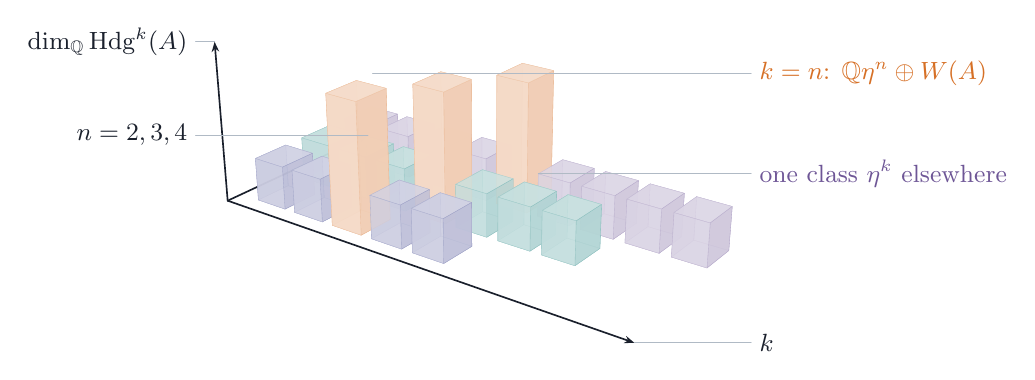
\begin{tikzpicture}[x=1cm,y=1cm,line join=round,line cap=round,
  font=\small,text=PInk]
  \path[draw=PViolet!41!white,line width=0.12pt,fill opacity=0.80,fill=PViolet!25!white] (-1.4437,0.2987) -- (-1.1159,0.2019) -- (-1.1295,0.6963) -- (-1.4611,0.7877) -- cycle;
  \path[draw=PViolet!50!white,line width=0.12pt,fill opacity=0.80,fill=PViolet!34!white] (-1.7743,0.1410) -- (-1.4437,0.2987) -- (-1.4611,0.7877) -- (-1.7961,0.6388) -- cycle;
  \path[draw=PViolet!39!white,line width=0.12pt,fill opacity=0.80,fill=PViolet!23!white] (-1.7743,0.1410) -- (-1.4439,0.0400) -- (-1.1159,0.2019) -- (-1.4437,0.2987) -- cycle;
  \path[draw=PViolet!39!white,line width=0.12pt,fill opacity=0.80,fill=PViolet!23!white] (-1.7961,0.6388) -- (-1.4618,0.5433) -- (-1.1295,0.6963) -- (-1.4611,0.7877) -- cycle;
  \path[draw=PViolet!50!white,line width=0.12pt,fill opacity=0.80,fill=PViolet!34!white] (-1.4439,0.0400) -- (-1.1159,0.2019) -- (-1.1295,0.6963) -- (-1.4618,0.5433) -- cycle;
  \path[draw=PViolet!41!white,line width=0.12pt,fill opacity=0.80,fill=PViolet!25!white] (-0.9981,0.1671) -- (-0.6584,0.0668) -- (-0.6666,0.5686) -- (-1.0104,0.6634) -- cycle;
  \path[draw=PViolet!41!white,line width=0.12pt,fill opacity=0.80,fill=PViolet!25!white] (-1.7743,0.1410) -- (-1.4439,0.0400) -- (-1.4618,0.5433) -- (-1.7961,0.6388) -- cycle;
  \path[draw=PViolet!50!white,line width=0.12pt,fill opacity=0.80,fill=PViolet!34!white] (-1.3251,0.0037) -- (-0.9981,0.1671) -- (-1.0104,0.6634) -- (-1.3417,0.5090) -- cycle;
  \path[draw=PViolet!39!white,line width=0.12pt,fill opacity=0.80,fill=PViolet!23!white] (-1.3251,0.0037) -- (-0.9823,-0.1011) -- (-0.6584,0.0668) -- (-0.9981,0.1671) -- cycle;
  \draw[PInk,line width=0.6pt,-{Stealth[length=3.6pt]}] (-3.2866,-0.4030) -- (-1.5062,0.4276);
  \path[draw=PTeal!41!white,line width=0.12pt,fill opacity=0.80,fill=PTeal!25!white] (-1.9623,0.0514) -- (-1.6304,-0.0521) -- (-1.6510,0.4562) -- (-1.9867,0.5541) -- cycle;
  \path[draw=PViolet!39!white,line width=0.12pt,fill opacity=0.80,fill=PViolet!23!white] (-1.3417,0.5090) -- (-0.9948,0.4099) -- (-0.6666,0.5686) -- (-1.0104,0.6634) -- cycle;
  \path[draw=PViolet!50!white,line width=0.12pt,fill opacity=0.80,fill=PViolet!34!white] (-0.9823,-0.1011) -- (-0.6584,0.0668) -- (-0.6666,0.5686) -- (-0.9948,0.4099) -- cycle;
  \path[draw=PViolet!41!white,line width=0.12pt,fill opacity=0.80,fill=PViolet!25!white] (-0.5363,0.0307) -- (-0.1840,-0.0734) -- (-0.1863,0.4361) -- (-0.5430,0.5345) -- cycle;
  \path[draw=PTeal!50!white,line width=0.12pt,fill opacity=0.80,fill=PTeal!34!white] (-2.3158,-0.1172) -- (-1.9623,0.0514) -- (-1.9867,0.5541) -- (-2.3453,0.3946) -- cycle;
  \path[draw=PTeal!39!white,line width=0.12pt,fill opacity=0.80,fill=PTeal!23!white] (-2.3158,-0.1172) -- (-1.9814,-0.2254) -- (-1.6304,-0.0521) -- (-1.9623,0.0514) -- cycle;
  \path[draw=PViolet!41!white,line width=0.12pt,fill opacity=0.80,fill=PViolet!25!white] (-1.3251,0.0037) -- (-0.9823,-0.1011) -- (-0.9948,0.4099) -- (-1.3417,0.5090) -- cycle;
  \path[draw=PViolet!50!white,line width=0.12pt,fill opacity=0.80,fill=PViolet!34!white] (-0.8591,-0.1388) -- (-0.5363,0.0307) -- (-0.5430,0.5345) -- (-0.8700,0.3742) -- cycle;
  \path[draw=PViolet!39!white,line width=0.12pt,fill opacity=0.80,fill=PViolet!23!white] (-0.8591,-0.1388) -- (-0.5033,-0.2476) -- (-0.1840,-0.0734) -- (-0.5363,0.0307) -- cycle;
  \path[draw=PTeal!39!white,line width=0.12pt,fill opacity=0.80,fill=PTeal!23!white] (-2.3453,0.3946) -- (-2.0070,0.2923) -- (-1.6510,0.4562) -- (-1.9867,0.5541) -- cycle;
  \path[draw=PTeal!50!white,line width=0.12pt,fill opacity=0.80,fill=PTeal!34!white] (-1.9814,-0.2254) -- (-1.6304,-0.0521) -- (-1.6510,0.4562) -- (-2.0070,0.2923) -- cycle;
  \path[draw=PTeal!41!white,line width=0.12pt,fill opacity=0.80,fill=PTeal!25!white] (-1.5111,-0.0893) -- (-1.1666,-0.1967) -- (-1.1816,0.3195) -- (-1.5302,0.4210) -- cycle;
  \path[draw=PViolet!39!white,line width=0.12pt,fill opacity=0.80,fill=PViolet!23!white] (-0.8700,0.3742) -- (-0.5098,0.2713) -- (-0.1863,0.4361) -- (-0.5430,0.5345) -- cycle;
  \path[draw=PViolet!50!white,line width=0.12pt,fill opacity=0.80,fill=PViolet!34!white] (-0.5033,-0.2476) -- (-0.1840,-0.0734) -- (-0.1863,0.4361) -- (-0.5098,0.2713) -- cycle;
  \path[draw=PViolet!41!white,line width=0.12pt,fill opacity=0.80,fill=PViolet!25!white] (-0.0573,-0.1108) -- (0.3084,-0.2188) -- (0.3123,0.2986) -- (-0.0580,0.4008) -- cycle;
  \path[draw=PTeal!41!white,line width=0.12pt,fill opacity=0.80,fill=PTeal!25!white] (-2.3158,-0.1172) -- (-1.9814,-0.2254) -- (-2.0070,0.2923) -- (-2.3453,0.3946) -- cycle;
  \path[draw=PTeal!50!white,line width=0.12pt,fill opacity=0.80,fill=PTeal!34!white] (-1.8611,-0.2643) -- (-1.5111,-0.0893) -- (-1.5302,0.4210) -- (-1.8852,0.2555) -- cycle;
  \path[draw=PTeal!39!white,line width=0.12pt,fill opacity=0.80,fill=PTeal!23!white] (-1.8611,-0.2643) -- (-1.5137,-0.3766) -- (-1.1666,-0.1967) -- (-1.5111,-0.0893) -- cycle;
  \path[draw=PViolet!41!white,line width=0.12pt,fill opacity=0.80,fill=PViolet!25!white] (-0.8591,-0.1388) -- (-0.5033,-0.2476) -- (-0.5098,0.2713) -- (-0.8700,0.3742) -- cycle;
  \path[draw=PViolet!50!white,line width=0.12pt,fill opacity=0.80,fill=PViolet!34!white] (-0.3753,-0.2867) -- (-0.0573,-0.1108) -- (-0.0580,0.4008) -- (-0.3802,0.2343) -- cycle;
  \path[draw=PViolet!39!white,line width=0.12pt,fill opacity=0.80,fill=PViolet!23!white] (-0.3753,-0.2867) -- (-0.0058,-0.3997) -- (0.3084,-0.2188) -- (-0.0573,-0.1108) -- cycle;
  \path[draw=PIndigo!41!white,line width=0.12pt,fill opacity=0.80,fill=PIndigo!25!white] (-2.5171,-0.2132) -- (-2.1813,-0.3241) -- (-2.2098,0.1989) -- (-2.5495,0.3039) -- cycle;
  \path[draw=PTeal!39!white,line width=0.12pt,fill opacity=0.80,fill=PTeal!23!white] (-1.8852,0.2555) -- (-1.5337,0.1492) -- (-1.1816,0.3195) -- (-1.5302,0.4210) -- cycle;
  \path[draw=PTeal!50!white,line width=0.12pt,fill opacity=0.80,fill=PTeal!34!white] (-1.5137,-0.3766) -- (-1.1666,-0.1967) -- (-1.1816,0.3195) -- (-1.5337,0.1492) -- cycle;
  \path[draw=PTeal!41!white,line width=0.12pt,fill opacity=0.80,fill=PTeal!25!white] (-1.0428,-0.2353) -- (-0.6851,-0.3468) -- (-0.6941,0.1774) -- (-1.0563,0.2829) -- cycle;
  \path[draw=PIndigo!50!white,line width=0.12pt,fill opacity=0.80,fill=PIndigo!34!white] (-2.8960,-0.3939) -- (-2.5171,-0.2132) -- (-2.5495,0.3039) -- (-2.9342,0.1329) -- cycle;
  \path[draw=PViolet!39!white,line width=0.12pt,fill opacity=0.80,fill=PViolet!23!white] (-0.3802,0.2343) -- (-0.0058,0.1273) -- (0.3123,0.2986) -- (-0.0580,0.4008) -- cycle;
  \path[draw=PIndigo!39!white,line width=0.12pt,fill opacity=0.80,fill=PIndigo!23!white] (-2.8960,-0.3939) -- (-2.5579,-0.5100) -- (-2.1813,-0.3241) -- (-2.5171,-0.2132) -- cycle;
  \path[draw=PViolet!50!white,line width=0.12pt,fill opacity=0.80,fill=PViolet!34!white] (-0.0058,-0.3997) -- (0.3084,-0.2188) -- (0.3123,0.2986) -- (-0.0058,0.1273) -- cycle;
  \path[draw=PTeal!41!white,line width=0.12pt,fill opacity=0.80,fill=PTeal!25!white] (-1.8611,-0.2643) -- (-1.5137,-0.3766) -- (-1.5337,0.1492) -- (-1.8852,0.2555) -- cycle;
  \path[draw=PTeal!50!white,line width=0.12pt,fill opacity=0.80,fill=PTeal!34!white] (-1.3888,-0.4171) -- (-1.0428,-0.2353) -- (-1.0563,0.2829) -- (-1.4071,0.1109) -- cycle;
  \path[draw=PTeal!39!white,line width=0.12pt,fill opacity=0.80,fill=PTeal!23!white] (-1.3888,-0.4171) -- (-1.0278,-0.5338) -- (-0.6851,-0.3468) -- (-1.0428,-0.2353) -- cycle;
  \path[draw=PViolet!41!white,line width=0.12pt,fill opacity=0.80,fill=PViolet!25!white] (-0.3753,-0.2867) -- (-0.0058,-0.3997) -- (-0.0058,0.1273) -- (-0.3802,0.2343) -- cycle;
  \path[draw=PAmber!39!white,line width=0.12pt,fill opacity=0.92,fill=PAmber!23!white] (0.1272,-0.4404) -- (0.5114,-0.5578) -- (0.8196,-0.3697) -- (0.4399,-0.2576) -- cycle;
  \path[draw=PIndigo!39!white,line width=0.12pt,fill opacity=0.80,fill=PIndigo!23!white] (-2.9342,0.1329) -- (-2.5921,0.0229) -- (-2.2098,0.1989) -- (-2.5495,0.3039) -- cycle;
  \path[draw=PIndigo!50!white,line width=0.12pt,fill opacity=0.80,fill=PIndigo!34!white] (-2.5579,-0.5100) -- (-2.1813,-0.3241) -- (-2.2098,0.1989) -- (-2.5921,0.0229) -- cycle;
  \path[draw=PAmber!41!white,line width=0.12pt,fill opacity=0.92,fill=PAmber!25!white] (0.4399,-0.2576) -- (0.8196,-0.3697) -- (0.8528,1.2491) -- (0.4574,1.3422) -- cycle;
  \path[draw=PIndigo!41!white,line width=0.12pt,fill opacity=0.80,fill=PIndigo!25!white] (-2.0605,-0.3640) -- (-1.7115,-0.4792) -- (-1.7343,0.0521) -- (-2.0875,0.1612) -- cycle;
  \path[draw=PTeal!39!white,line width=0.12pt,fill opacity=0.80,fill=PTeal!23!white] (-1.4071,0.1109) -- (-1.0415,0.0003) -- (-0.6941,0.1774) -- (-1.0563,0.2829) -- cycle;
  \path[draw=PTeal!50!white,line width=0.12pt,fill opacity=0.80,fill=PTeal!34!white] (-1.0278,-0.5338) -- (-0.6851,-0.3468) -- (-0.6941,0.1774) -- (-1.0415,0.0003) -- cycle;
  \path[draw=PIndigo!41!white,line width=0.12pt,fill opacity=0.80,fill=PIndigo!25!white] (-2.8960,-0.3939) -- (-2.5579,-0.5100) -- (-2.5921,0.0229) -- (-2.9342,0.1329) -- cycle;
  \path[draw=PAmber!50!white,line width=0.12pt,fill opacity=0.92,fill=PAmber!34!white] (0.1272,-0.4404) -- (0.4399,-0.2576) -- (0.4574,1.3422) -- (0.1324,1.1905) -- cycle;
  \path[draw=PIndigo!50!white,line width=0.12pt,fill opacity=0.80,fill=PIndigo!34!white] (-2.4362,-0.5517) -- (-2.0605,-0.3640) -- (-2.0875,0.1612) -- (-2.4689,-0.0166) -- cycle;
  \path[draw=PIndigo!39!white,line width=0.12pt,fill opacity=0.80,fill=PIndigo!23!white] (-2.4362,-0.5517) -- (-2.0845,-0.6725) -- (-1.7115,-0.4792) -- (-2.0605,-0.3640) -- cycle;
  \path[draw=PViolet!41!white,line width=0.12pt,fill opacity=0.80,fill=PViolet!25!white] (0.9563,-0.4101) -- (1.3510,-0.5266) -- (1.3691,0.0071) -- (0.9689,0.1175) -- cycle;
  \path[draw=PTeal!41!white,line width=0.12pt,fill opacity=0.80,fill=PTeal!25!white] (-1.3888,-0.4171) -- (-1.0278,-0.5338) -- (-1.0415,0.0003) -- (-1.4071,0.1109) -- cycle;
  \path[draw=PAmber!39!white,line width=0.12pt,fill opacity=0.92,fill=PAmber!23!white] (-0.8978,-0.5758) -- (-0.5223,-0.6973) -- (-0.1848,-0.5028) -- (-0.5565,-0.3870) -- cycle;
  \path[draw=PViolet!50!white,line width=0.12pt,fill opacity=0.80,fill=PViolet!34!white] (0.6496,-0.6001) -- (0.9563,-0.4101) -- (0.9689,0.1175) -- (0.6584,-0.0624) -- cycle;
  \path[draw=PViolet!39!white,line width=0.12pt,fill opacity=0.80,fill=PViolet!23!white] (0.6496,-0.6001) -- (1.0492,-0.7223) -- (1.3510,-0.5266) -- (0.9563,-0.4101) -- cycle;
  \draw[PInk,line width=0.6pt,-{Stealth[length=3.6pt]}] (-3.2866,-0.4030) -- (-3.4526,1.6143);
  \path[draw=PAmber!41!white,line width=0.12pt,fill opacity=0.92,fill=PAmber!25!white] (-0.5565,-0.3870) -- (-0.1848,-0.5028) -- (-0.1924,1.1386) -- (-0.5790,1.2349) -- cycle;
  \path[draw=PIndigo!39!white,line width=0.12pt,fill opacity=0.80,fill=PIndigo!23!white] (-2.4689,-0.0166) -- (-2.1129,-0.1310) -- (-1.7343,0.0521) -- (-2.0875,0.1612) -- cycle;
  \path[draw=PAmber!50!white,line width=0.12pt,fill opacity=0.92,fill=PAmber!34!white] (0.5114,-0.5578) -- (0.8196,-0.3697) -- (0.8528,1.2491) -- (0.5326,1.0929) -- cycle;
  \path[draw=PIndigo!50!white,line width=0.12pt,fill opacity=0.80,fill=PIndigo!34!white] (-2.0845,-0.6725) -- (-1.7115,-0.4792) -- (-1.7343,0.0521) -- (-2.1129,-0.1310) -- cycle;
  \path[draw=PAmber!50!white,line width=0.12pt,fill opacity=0.92,fill=PAmber!34!white] (-0.8978,-0.5758) -- (-0.5565,-0.3870) -- (-0.5790,1.2349) -- (-0.9351,1.0779) -- cycle;
  \path[draw=PTeal!41!white,line width=0.12pt,fill opacity=0.80,fill=PTeal!25!white] (-0.0510,-0.5445) -- (0.3355,-0.6651) -- (0.3401,-0.1240) -- (-0.0517,-0.0098) -- cycle;
  \path[draw=PAmber!41!white,line width=0.12pt,fill opacity=0.92,fill=PAmber!25!white] (0.1272,-0.4404) -- (0.5114,-0.5578) -- (0.5326,1.0929) -- (0.1324,1.1905) -- cycle;
  \path[draw=PIndigo!41!white,line width=0.12pt,fill opacity=0.80,fill=PIndigo!25!white] (-2.4362,-0.5517) -- (-2.0845,-0.6725) -- (-2.1129,-0.1310) -- (-2.4689,-0.0166) -- cycle;
  \path[draw=PViolet!39!white,line width=0.12pt,fill opacity=0.80,fill=PViolet!23!white] (0.6584,-0.0624) -- (1.0636,-0.1782) -- (1.3691,0.0071) -- (0.9689,0.1175) -- cycle;
  \path[draw=PAmber!39!white,line width=0.12pt,fill opacity=0.92,fill=PAmber!23!white] (-1.9578,-0.7159) -- (-1.5918,-0.8416) -- (-1.2231,-0.6404) -- (-1.5860,-0.5206) -- cycle;
  \path[draw=PViolet!50!white,line width=0.12pt,fill opacity=0.80,fill=PViolet!34!white] (1.0492,-0.7223) -- (1.3510,-0.5266) -- (1.3691,0.0071) -- (1.0636,-0.1782) -- cycle;
  \path[draw=PViolet!41!white,line width=0.12pt,fill opacity=0.80,fill=PViolet!25!white] (1.4930,-0.5686) -- (1.9035,-0.6898) -- (1.9296,-0.1475) -- (1.5131,-0.0326) -- cycle;
  \path[draw=PTeal!50!white,line width=0.12pt,fill opacity=0.80,fill=PTeal!34!white] (-0.3871,-0.7410) -- (-0.0510,-0.5445) -- (-0.0517,-0.0098) -- (-0.3924,-0.1960) -- cycle;
  \path[draw=PTeal!39!white,line width=0.12pt,fill opacity=0.80,fill=PTeal!23!white] (-0.3871,-0.7410) -- (0.0038,-0.8674) -- (0.3355,-0.6651) -- (-0.0510,-0.5445) -- cycle;
  \path[draw=PViolet!41!white,line width=0.12pt,fill opacity=0.80,fill=PViolet!25!white] (0.6496,-0.6001) -- (1.0492,-0.7223) -- (1.0636,-0.1782) -- (0.6584,-0.0624) -- cycle;
  \path[draw=PViolet!50!white,line width=0.12pt,fill opacity=0.80,fill=PViolet!34!white] (1.1931,-0.7662) -- (1.4930,-0.5686) -- (1.5131,-0.0326) -- (1.2096,-0.2199) -- cycle;
  \path[draw=PViolet!39!white,line width=0.12pt,fill opacity=0.80,fill=PViolet!23!white] (1.1931,-0.7662) -- (1.6091,-0.8934) -- (1.9035,-0.6898) -- (1.4930,-0.5686) -- cycle;
  \path[draw=PAmber!39!white,line width=0.12pt,fill opacity=0.92,fill=PAmber!23!white] (0.1324,1.1905) -- (0.5326,1.0929) -- (0.8528,1.2491) -- (0.4574,1.3422) -- cycle;
  \path[draw=PAmber!41!white,line width=0.12pt,fill opacity=0.92,fill=PAmber!25!white] (-1.5860,-0.5206) -- (-1.2231,-0.6404) -- (-1.2744,1.0242) -- (-1.6515,1.1238) -- cycle;
  \path[draw=PAmber!50!white,line width=0.12pt,fill opacity=0.92,fill=PAmber!34!white] (-0.5223,-0.6973) -- (-0.1848,-0.5028) -- (-0.1924,1.1386) -- (-0.5443,0.9768) -- cycle;
  \path[draw=PAmber!50!white,line width=0.12pt,fill opacity=0.92,fill=PAmber!34!white] (-1.9578,-0.7159) -- (-1.5860,-0.5206) -- (-1.6515,1.1238) -- (-2.0407,0.9613) -- cycle;
  \path[draw=PIndigo!41!white,line width=0.12pt,fill opacity=0.80,fill=PIndigo!25!white] (-1.0925,-0.6836) -- (-0.7149,-0.8083) -- (-0.7248,-0.2597) -- (-1.1074,-0.1415) -- cycle;
  \path[draw=PAmber!41!white,line width=0.12pt,fill opacity=0.92,fill=PAmber!25!white] (-0.8978,-0.5758) -- (-0.5223,-0.6973) -- (-0.5443,0.9768) -- (-0.9351,1.0779) -- cycle;
  \path[draw=PTeal!39!white,line width=0.12pt,fill opacity=0.80,fill=PTeal!23!white] (-0.3924,-0.1960) -- (0.0039,-0.3158) -- (0.3401,-0.1240) -- (-0.0517,-0.0098) -- cycle;
  \path[draw=PTeal!50!white,line width=0.12pt,fill opacity=0.80,fill=PTeal!34!white] (0.0038,-0.8674) -- (0.3355,-0.6651) -- (0.3401,-0.1240) -- (0.0039,-0.3158) -- cycle;
  \path[draw=PTeal!41!white,line width=0.12pt,fill opacity=0.80,fill=PTeal!25!white] (0.4747,-0.7085) -- (0.8770,-0.8339) -- (0.8892,-0.2840) -- (0.4812,-0.1651) -- cycle;
  \path[draw=PIndigo!50!white,line width=0.12pt,fill opacity=0.80,fill=PIndigo!34!white] (-1.4599,-0.8869) -- (-1.0925,-0.6836) -- (-1.1074,-0.1415) -- (-1.4804,-0.3342) -- cycle;
  \path[draw=PViolet!39!white,line width=0.12pt,fill opacity=0.80,fill=PViolet!23!white] (1.2096,-0.2199) -- (1.6317,-0.3405) -- (1.9296,-0.1475) -- (1.5131,-0.0326) -- cycle;
  \path[draw=PIndigo!39!white,line width=0.12pt,fill opacity=0.80,fill=PIndigo!23!white] (-1.4599,-0.8869) -- (-1.0786,-1.0178) -- (-0.7149,-0.8083) -- (-1.0925,-0.6836) -- cycle;
  \path[draw=PViolet!50!white,line width=0.12pt,fill opacity=0.80,fill=PViolet!34!white] (1.6091,-0.8934) -- (1.9035,-0.6898) -- (1.9296,-0.1475) -- (1.6317,-0.3405) -- cycle;
  \path[draw=PViolet!41!white,line width=0.12pt,fill opacity=0.80,fill=PViolet!25!white] (2.0513,-0.7335) -- (2.4787,-0.8597) -- (2.5132,-0.3085) -- (2.0795,-0.1888) -- cycle;
  \path[draw=PTeal!41!white,line width=0.12pt,fill opacity=0.80,fill=PTeal!25!white] (-0.3871,-0.7410) -- (0.0038,-0.8674) -- (0.0039,-0.3158) -- (-0.3924,-0.1960) -- cycle;
  \path[draw=PTeal!50!white,line width=0.12pt,fill opacity=0.80,fill=PTeal!34!white] (0.1446,-0.9130) -- (0.4747,-0.7085) -- (0.4812,-0.1651) -- (0.1466,-0.3590) -- cycle;
  \path[draw=PTeal!39!white,line width=0.12pt,fill opacity=0.80,fill=PTeal!23!white] (0.1446,-0.9130) -- (0.5518,-1.0447) -- (0.8770,-0.8339) -- (0.4747,-0.7085) -- cycle;
  \path[draw=PAmber!39!white,line width=0.12pt,fill opacity=0.92,fill=PAmber!23!white] (-0.9351,1.0779) -- (-0.5443,0.9768) -- (-0.1924,1.1386) -- (-0.5790,1.2349) -- cycle;
  \path[draw=PViolet!41!white,line width=0.12pt,fill opacity=0.80,fill=PViolet!25!white] (1.1931,-0.7662) -- (1.6091,-0.8934) -- (1.6317,-0.3405) -- (1.2096,-0.2199) -- cycle;
  \path[draw=PViolet!50!white,line width=0.12pt,fill opacity=0.80,fill=PViolet!34!white] (1.7590,-0.9393) -- (2.0513,-0.7335) -- (2.0795,-0.1888) -- (1.7838,-0.3839) -- cycle;
  \path[draw=PViolet!39!white,line width=0.12pt,fill opacity=0.80,fill=PViolet!23!white] (1.7590,-0.9393) -- (2.1925,-1.0718) -- (2.4787,-0.8597) -- (2.0513,-0.7335) -- cycle;
  \path[draw=PAmber!50!white,line width=0.12pt,fill opacity=0.92,fill=PAmber!34!white] (-1.5918,-0.8416) -- (-1.2231,-0.6404) -- (-1.2744,1.0242) -- (-1.6602,0.8566) -- cycle;
  \path[draw=PAmber!41!white,line width=0.12pt,fill opacity=0.92,fill=PAmber!25!white] (-1.9578,-0.7159) -- (-1.5918,-0.8416) -- (-1.6602,0.8566) -- (-2.0407,0.9613) -- cycle;
  \path[draw=PIndigo!39!white,line width=0.12pt,fill opacity=0.80,fill=PIndigo!23!white] (-1.4804,-0.3342) -- (-1.0939,-0.4584) -- (-0.7248,-0.2597) -- (-1.1074,-0.1415) -- cycle;
  \path[draw=PIndigo!50!white,line width=0.12pt,fill opacity=0.80,fill=PIndigo!34!white] (-1.0786,-1.0178) -- (-0.7149,-0.8083) -- (-0.7248,-0.2597) -- (-1.0939,-0.4584) -- cycle;
  \path[draw=PIndigo!41!white,line width=0.12pt,fill opacity=0.80,fill=PIndigo!25!white] (-0.5789,-0.8532) -- (-0.1856,-0.9830) -- (-0.1883,-0.4254) -- (-0.5870,-0.3023) -- cycle;
  \path[draw=PTeal!39!white,line width=0.12pt,fill opacity=0.80,fill=PTeal!23!white] (0.1466,-0.3590) -- (0.5597,-0.4839) -- (0.8892,-0.2840) -- (0.4812,-0.1651) -- cycle;
  \path[draw=PTeal!50!white,line width=0.12pt,fill opacity=0.80,fill=PTeal!34!white] (0.5518,-1.0447) -- (0.8770,-0.8339) -- (0.8892,-0.2840) -- (0.5597,-0.4839) -- cycle;
  \path[draw=PTeal!41!white,line width=0.12pt,fill opacity=0.80,fill=PTeal!25!white] (1.0219,-0.8791) -- (1.4410,-1.0097) -- (1.4615,-0.4508) -- (1.0362,-0.3268) -- cycle;
  \path[draw=PIndigo!41!white,line width=0.12pt,fill opacity=0.80,fill=PIndigo!25!white] (-1.4599,-0.8869) -- (-1.0786,-1.0178) -- (-1.0939,-0.4584) -- (-1.4804,-0.3342) -- cycle;
  \path[draw=PIndigo!50!white,line width=0.12pt,fill opacity=0.80,fill=PIndigo!34!white] (-0.9412,-1.0649) -- (-0.5789,-0.8532) -- (-0.5870,-0.3023) -- (-0.9546,-0.5031) -- cycle;
  \path[draw=PViolet!39!white,line width=0.12pt,fill opacity=0.80,fill=PViolet!23!white] (1.7838,-0.3839) -- (2.2238,-0.5096) -- (2.5132,-0.3085) -- (2.0795,-0.1888) -- cycle;
  \path[draw=PIndigo!39!white,line width=0.12pt,fill opacity=0.80,fill=PIndigo!23!white] (-0.9412,-1.0649) -- (-0.5436,-1.2014) -- (-0.1856,-0.9830) -- (-0.5789,-0.8532) -- cycle;
  \path[draw=PViolet!50!white,line width=0.12pt,fill opacity=0.80,fill=PViolet!34!white] (2.1925,-1.0718) -- (2.4787,-0.8597) -- (2.5132,-0.3085) -- (2.2238,-0.5096) -- cycle;
  \path[draw=PAmber!39!white,line width=0.12pt,fill opacity=0.92,fill=PAmber!23!white] (-2.0407,0.9613) -- (-1.6602,0.8566) -- (-1.2744,1.0242) -- (-1.6515,1.1238) -- cycle;
  \path[draw=PViolet!41!white,line width=0.12pt,fill opacity=0.80,fill=PViolet!25!white] (2.6326,-0.9051) -- (3.0777,-1.0366) -- (3.1216,-0.4763) -- (2.6695,-0.3516) -- cycle;
  \path[draw=PTeal!41!white,line width=0.12pt,fill opacity=0.80,fill=PTeal!25!white] (0.1446,-0.9130) -- (0.5518,-1.0447) -- (0.5597,-0.4839) -- (0.1466,-0.3590) -- cycle;
  \path[draw=PTeal!50!white,line width=0.12pt,fill opacity=0.80,fill=PTeal!34!white] (0.6986,-1.0922) -- (1.0219,-0.8791) -- (1.0362,-0.3268) -- (0.7086,-0.5290) -- cycle;
  \path[draw=PTeal!39!white,line width=0.12pt,fill opacity=0.80,fill=PTeal!23!white] (0.6986,-1.0922) -- (1.1232,-1.2295) -- (1.4410,-1.0097) -- (1.0219,-0.8791) -- cycle;
  \path[draw=PViolet!41!white,line width=0.12pt,fill opacity=0.80,fill=PViolet!25!white] (1.7590,-0.9393) -- (2.1925,-1.0718) -- (2.2238,-0.5096) -- (1.7838,-0.3839) -- cycle;
  \path[draw=PViolet!50!white,line width=0.12pt,fill opacity=0.80,fill=PViolet!34!white] (2.3487,-1.1195) -- (2.6326,-0.9051) -- (2.6695,-0.3516) -- (2.3825,-0.5550) -- cycle;
  \path[draw=PViolet!39!white,line width=0.12pt,fill opacity=0.80,fill=PViolet!23!white] (2.3487,-1.1195) -- (2.8007,-1.2578) -- (3.0777,-1.0366) -- (2.6326,-0.9051) -- cycle;
  \path[draw=PIndigo!39!white,line width=0.12pt,fill opacity=0.80,fill=PIndigo!23!white] (-0.9546,-0.5031) -- (-0.5515,-0.6327) -- (-0.1883,-0.4254) -- (-0.5870,-0.3023) -- cycle;
  \path[draw=PIndigo!50!white,line width=0.12pt,fill opacity=0.80,fill=PIndigo!34!white] (-0.5436,-1.2014) -- (-0.1856,-0.9830) -- (-0.1883,-0.4254) -- (-0.5515,-0.6327) -- cycle;
  \path[draw=PTeal!39!white,line width=0.12pt,fill opacity=0.80,fill=PTeal!23!white] (0.7086,-0.5290) -- (1.1396,-0.6593) -- (1.4615,-0.4508) -- (1.0362,-0.3268) -- cycle;
  \path[draw=PTeal!50!white,line width=0.12pt,fill opacity=0.80,fill=PTeal!34!white] (1.1232,-1.2295) -- (1.4410,-1.0097) -- (1.4615,-0.4508) -- (1.1396,-0.6593) -- cycle;
  \path[draw=PIndigo!41!white,line width=0.12pt,fill opacity=0.80,fill=PIndigo!25!white] (-0.9412,-1.0649) -- (-0.5436,-1.2014) -- (-0.5515,-0.6327) -- (-0.9546,-0.5031) -- cycle;
  \path[draw=PViolet!39!white,line width=0.12pt,fill opacity=0.80,fill=PViolet!23!white] (2.3825,-0.5550) -- (2.8417,-0.6861) -- (3.1216,-0.4763) -- (2.6695,-0.3516) -- cycle;
  \path[draw=PViolet!50!white,line width=0.12pt,fill opacity=0.80,fill=PViolet!34!white] (2.8007,-1.2578) -- (3.0777,-1.0366) -- (3.1216,-0.4763) -- (2.8417,-0.6861) -- cycle;
  \draw[PInk,line width=0.6pt,-{Stealth[length=3.6pt]}] (-3.2866,-0.4030) -- (1.8787,-2.2084);
  \path[draw=PTeal!41!white,line width=0.12pt,fill opacity=0.80,fill=PTeal!25!white] (0.6986,-1.0922) -- (1.1232,-1.2295) -- (1.1396,-0.6593) -- (0.7086,-0.5290) -- cycle;
  \path[draw=PViolet!41!white,line width=0.12pt,fill opacity=0.80,fill=PViolet!25!white] (2.3487,-1.1195) -- (2.8007,-1.2578) -- (2.8417,-0.6861) -- (2.3825,-0.5550) -- cycle;
  \draw[PRule,line width=0.35pt] (-3.6926,1.6143) -- (-3.4526,1.6143);
  \node[anchor=east,inner sep=0pt] at (-3.7926,1.6143) {$\dim_{\QQ}\Hdg^{k}(A)$};
  \draw[PRule,line width=0.35pt] (-3.6926,0.4276) -- (-1.5062,0.4276);
  \node[anchor=east,inner sep=0pt] at (-3.7926,0.4276) {$n=2,3,4$};
  \draw[PRule,line width=0.35pt] (3.3616,1.2099) -- (-1.4454,1.2099);
  \node[text=PAmber,anchor=west,inner sep=0pt] at (3.4616,1.2099) {$k=n$: $\QQ\eta^{n}\oplus W(A)$};
  \draw[PRule,line width=0.35pt] (3.3616,-0.0624) -- (0.6584,-0.0624);
  \node[text=PViolet,anchor=west,inner sep=0pt] at (3.4616,-0.0624) {one class $\eta^{k}$ elsewhere};
  \draw[PRule,line width=0.35pt] (3.3616,-2.2084) -- (1.8787,-2.2084);
  \node[anchor=west,inner sep=0pt] at (3.4616,-2.2084) {$k$};
\end{tikzpicture}
\end{document}
